\documentclass{article}
% translate with >> pdflatex -shell-escape <file>

% This file is an extract of the PGFPLOTS manual, copyright by Christian Feuersaenger.
% 
% Feel free to use it as long as you cite the pgfplots manual properly.
%
% See
%   http://pgfplots.sourceforge.net/pgfplots.pdf
% for the complete manual.
%
% Any required input files (for <plot table> or <plot file> or the table package) can be downloaded
% at
% http://www.ctan.org/tex-archive/graphics/pgf/contrib/pgfplots/doc/latex/
% and
% http://www.ctan.org/tex-archive/graphics/pgf/contrib/pgfplots/doc/latex/plotdata/

\usepackage{pgfplots}
\pgfplotsset{compat=newest}

\pagestyle{empty}

\begin{document}
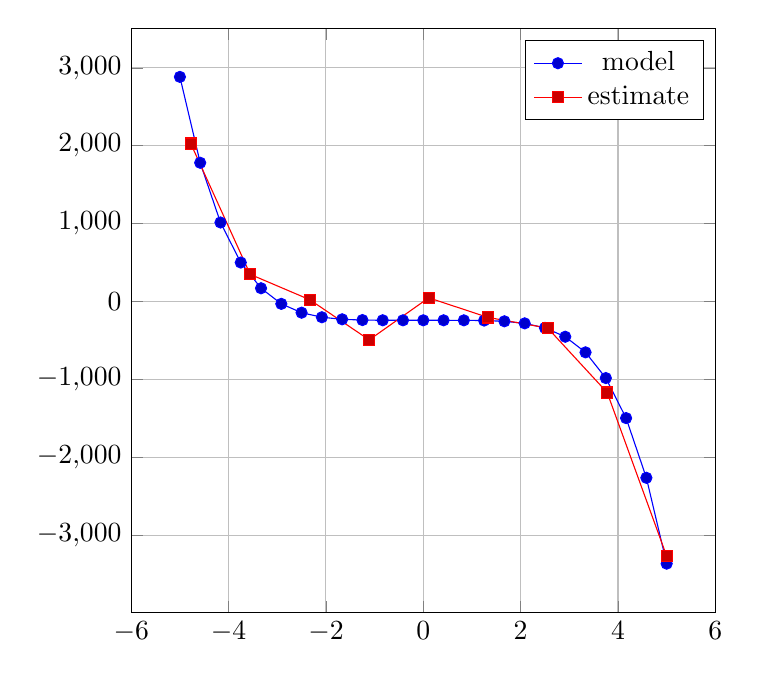
\begin{tikzpicture}
	\begin{axis}[
		height=9cm,
		width=9cm,
		grid=major,
	]
		
	\addplot {-x^5 - 242};
	\addlegendentry{model}

	\addplot coordinates {
		(-4.77778,2027.60977)
		(-3.55556,347.84069)
		(-2.33333,22.58953)
		(-1.11111,-493.50066)
		(0.11111,46.66082)
		(1.33333,-205.56286)
		(2.55556,-341.40638)
		(3.77778,-1169.24780)
		(5.00000,-3269.56775)
	};
	\addlegendentry{estimate}
	\end{axis}
\end{tikzpicture}
\end{document}
